% Options for packages loaded elsewhere
\PassOptionsToPackage{unicode}{hyperref}
\PassOptionsToPackage{hyphens}{url}
%
\documentclass[
]{article}
\usepackage{amsmath,amssymb}
\usepackage{lmodern}
\usepackage{iftex}
\ifPDFTeX
  \usepackage[T1]{fontenc}
  \usepackage[utf8]{inputenc}
  \usepackage{textcomp} % provide euro and other symbols
\else % if luatex or xetex
  \usepackage{unicode-math}
  \defaultfontfeatures{Scale=MatchLowercase}
  \defaultfontfeatures[\rmfamily]{Ligatures=TeX,Scale=1}
\fi
% Use upquote if available, for straight quotes in verbatim environments
\IfFileExists{upquote.sty}{\usepackage{upquote}}{}
\IfFileExists{microtype.sty}{% use microtype if available
  \usepackage[]{microtype}
  \UseMicrotypeSet[protrusion]{basicmath} % disable protrusion for tt fonts
}{}
\makeatletter
\@ifundefined{KOMAClassName}{% if non-KOMA class
  \IfFileExists{parskip.sty}{%
    \usepackage{parskip}
  }{% else
    \setlength{\parindent}{0pt}
    \setlength{\parskip}{6pt plus 2pt minus 1pt}}
}{% if KOMA class
  \KOMAoptions{parskip=half}}
\makeatother
\usepackage{xcolor}
\IfFileExists{xurl.sty}{\usepackage{xurl}}{} % add URL line breaks if available
\IfFileExists{bookmark.sty}{\usepackage{bookmark}}{\usepackage{hyperref}}
\hypersetup{
  pdftitle={Project\_1\_Reproducible Researh},
  pdfauthor={Dodanim},
  hidelinks,
  pdfcreator={LaTeX via pandoc}}
\urlstyle{same} % disable monospaced font for URLs
\usepackage[margin=1in]{geometry}
\usepackage{color}
\usepackage{fancyvrb}
\newcommand{\VerbBar}{|}
\newcommand{\VERB}{\Verb[commandchars=\\\{\}]}
\DefineVerbatimEnvironment{Highlighting}{Verbatim}{commandchars=\\\{\}}
% Add ',fontsize=\small' for more characters per line
\usepackage{framed}
\definecolor{shadecolor}{RGB}{248,248,248}
\newenvironment{Shaded}{\begin{snugshade}}{\end{snugshade}}
\newcommand{\AlertTok}[1]{\textcolor[rgb]{0.94,0.16,0.16}{#1}}
\newcommand{\AnnotationTok}[1]{\textcolor[rgb]{0.56,0.35,0.01}{\textbf{\textit{#1}}}}
\newcommand{\AttributeTok}[1]{\textcolor[rgb]{0.77,0.63,0.00}{#1}}
\newcommand{\BaseNTok}[1]{\textcolor[rgb]{0.00,0.00,0.81}{#1}}
\newcommand{\BuiltInTok}[1]{#1}
\newcommand{\CharTok}[1]{\textcolor[rgb]{0.31,0.60,0.02}{#1}}
\newcommand{\CommentTok}[1]{\textcolor[rgb]{0.56,0.35,0.01}{\textit{#1}}}
\newcommand{\CommentVarTok}[1]{\textcolor[rgb]{0.56,0.35,0.01}{\textbf{\textit{#1}}}}
\newcommand{\ConstantTok}[1]{\textcolor[rgb]{0.00,0.00,0.00}{#1}}
\newcommand{\ControlFlowTok}[1]{\textcolor[rgb]{0.13,0.29,0.53}{\textbf{#1}}}
\newcommand{\DataTypeTok}[1]{\textcolor[rgb]{0.13,0.29,0.53}{#1}}
\newcommand{\DecValTok}[1]{\textcolor[rgb]{0.00,0.00,0.81}{#1}}
\newcommand{\DocumentationTok}[1]{\textcolor[rgb]{0.56,0.35,0.01}{\textbf{\textit{#1}}}}
\newcommand{\ErrorTok}[1]{\textcolor[rgb]{0.64,0.00,0.00}{\textbf{#1}}}
\newcommand{\ExtensionTok}[1]{#1}
\newcommand{\FloatTok}[1]{\textcolor[rgb]{0.00,0.00,0.81}{#1}}
\newcommand{\FunctionTok}[1]{\textcolor[rgb]{0.00,0.00,0.00}{#1}}
\newcommand{\ImportTok}[1]{#1}
\newcommand{\InformationTok}[1]{\textcolor[rgb]{0.56,0.35,0.01}{\textbf{\textit{#1}}}}
\newcommand{\KeywordTok}[1]{\textcolor[rgb]{0.13,0.29,0.53}{\textbf{#1}}}
\newcommand{\NormalTok}[1]{#1}
\newcommand{\OperatorTok}[1]{\textcolor[rgb]{0.81,0.36,0.00}{\textbf{#1}}}
\newcommand{\OtherTok}[1]{\textcolor[rgb]{0.56,0.35,0.01}{#1}}
\newcommand{\PreprocessorTok}[1]{\textcolor[rgb]{0.56,0.35,0.01}{\textit{#1}}}
\newcommand{\RegionMarkerTok}[1]{#1}
\newcommand{\SpecialCharTok}[1]{\textcolor[rgb]{0.00,0.00,0.00}{#1}}
\newcommand{\SpecialStringTok}[1]{\textcolor[rgb]{0.31,0.60,0.02}{#1}}
\newcommand{\StringTok}[1]{\textcolor[rgb]{0.31,0.60,0.02}{#1}}
\newcommand{\VariableTok}[1]{\textcolor[rgb]{0.00,0.00,0.00}{#1}}
\newcommand{\VerbatimStringTok}[1]{\textcolor[rgb]{0.31,0.60,0.02}{#1}}
\newcommand{\WarningTok}[1]{\textcolor[rgb]{0.56,0.35,0.01}{\textbf{\textit{#1}}}}
\usepackage{graphicx}
\makeatletter
\def\maxwidth{\ifdim\Gin@nat@width>\linewidth\linewidth\else\Gin@nat@width\fi}
\def\maxheight{\ifdim\Gin@nat@height>\textheight\textheight\else\Gin@nat@height\fi}
\makeatother
% Scale images if necessary, so that they will not overflow the page
% margins by default, and it is still possible to overwrite the defaults
% using explicit options in \includegraphics[width, height, ...]{}
\setkeys{Gin}{width=\maxwidth,height=\maxheight,keepaspectratio}
% Set default figure placement to htbp
\makeatletter
\def\fps@figure{htbp}
\makeatother
\setlength{\emergencystretch}{3em} % prevent overfull lines
\providecommand{\tightlist}{%
  \setlength{\itemsep}{0pt}\setlength{\parskip}{0pt}}
\setcounter{secnumdepth}{-\maxdimen} % remove section numbering
\ifLuaTeX
  \usepackage{selnolig}  % disable illegal ligatures
\fi

\title{Project\_1\_Reproducible Researh}
\author{Dodanim}
\date{2022-06-19}

\begin{document}
\maketitle

\hypertarget{first-step-load-data}{%
\subsection{First step: load data}\label{first-step-load-data}}

Loading and preprocessing the data Show any code that is needed to

\begin{itemize}
\item
  Load the data
\item
  Process/transform the data (if necessary) into a format suitable for
  your analysis
\end{itemize}

\begin{Shaded}
\begin{Highlighting}[]
\NormalTok{datos }\OtherTok{\textless{}{-}} \FunctionTok{read.csv}\NormalTok{(}\StringTok{"activity.csv"}\NormalTok{)}
\FunctionTok{head}\NormalTok{(datos)}
\end{Highlighting}
\end{Shaded}

\begin{verbatim}
##   steps       date interval
## 1    NA 2012-10-01        0
## 2    NA 2012-10-01        5
## 3    NA 2012-10-01       10
## 4    NA 2012-10-01       15
## 5    NA 2012-10-01       20
## 6    NA 2012-10-01       25
\end{verbatim}

\begin{Shaded}
\begin{Highlighting}[]
\FunctionTok{str}\NormalTok{(datos)}
\end{Highlighting}
\end{Shaded}

\begin{verbatim}
## 'data.frame':    17568 obs. of  3 variables:
##  $ steps   : int  NA NA NA NA NA NA NA NA NA NA ...
##  $ date    : chr  "2012-10-01" "2012-10-01" "2012-10-01" "2012-10-01" ...
##  $ interval: int  0 5 10 15 20 25 30 35 40 45 ...
\end{verbatim}

\begin{Shaded}
\begin{Highlighting}[]
\FunctionTok{summary}\NormalTok{(datos)}
\end{Highlighting}
\end{Shaded}

\begin{verbatim}
##      steps            date              interval     
##  Min.   :  0.00   Length:17568       Min.   :   0.0  
##  1st Qu.:  0.00   Class :character   1st Qu.: 588.8  
##  Median :  0.00   Mode  :character   Median :1177.5  
##  Mean   : 37.38                      Mean   :1177.5  
##  3rd Qu.: 12.00                      3rd Qu.:1766.2  
##  Max.   :806.00                      Max.   :2355.0  
##  NA's   :2304
\end{verbatim}

\hypertarget{procesing-data-and-cleaning}{%
\subsubsection{Procesing data and
cleaning}\label{procesing-data-and-cleaning}}

\begin{Shaded}
\begin{Highlighting}[]
\NormalTok{datos}\SpecialCharTok{$}\NormalTok{day }\OtherTok{\textless{}{-}} \FunctionTok{weekdays}\NormalTok{(}\FunctionTok{as.Date}\NormalTok{(datos}\SpecialCharTok{$}\NormalTok{date))}
\NormalTok{datos}\SpecialCharTok{$}\NormalTok{date }\OtherTok{\textless{}{-}} \FunctionTok{as.POSIXct}\NormalTok{(datos}\SpecialCharTok{$}\NormalTok{date, }\AttributeTok{format =} \StringTok{"\%Y{-}\%m{-}\%d"}\NormalTok{)}

\NormalTok{datos\_limpios }\OtherTok{\textless{}{-}}\NormalTok{ datos[}\SpecialCharTok{!}\FunctionTok{is.na}\NormalTok{(datos}\SpecialCharTok{$}\NormalTok{steps),]}
\FunctionTok{head}\NormalTok{(datos\_limpios)}
\end{Highlighting}
\end{Shaded}

\begin{verbatim}
##     steps       date interval     day
## 289     0 2012-10-02        0 Tuesday
## 290     0 2012-10-02        5 Tuesday
## 291     0 2012-10-02       10 Tuesday
## 292     0 2012-10-02       15 Tuesday
## 293     0 2012-10-02       20 Tuesday
## 294     0 2012-10-02       25 Tuesday
\end{verbatim}

\hypertarget{what-is-the-average-daily-activity-pattern}{%
\subsection{What is the average daily activity
pattern?}\label{what-is-the-average-daily-activity-pattern}}

\hypertarget{calculate-the-total-number-of-steps-taken-per-day-ignore-the-missing-values}{%
\paragraph{1. Calculate the total number of steps taken per day (ignore
the missing
values)}\label{calculate-the-total-number-of-steps-taken-per-day-ignore-the-missing-values}}

\begin{Shaded}
\begin{Highlighting}[]
\NormalTok{sumTable }\OtherTok{\textless{}{-}} \FunctionTok{aggregate}\NormalTok{(datos}\SpecialCharTok{$}\NormalTok{steps }\SpecialCharTok{\textasciitilde{}}\NormalTok{ datos}\SpecialCharTok{$}\NormalTok{date, }\AttributeTok{FUN=}\NormalTok{sum, )}
\FunctionTok{colnames}\NormalTok{(sumTable)}\OtherTok{\textless{}{-}} \FunctionTok{c}\NormalTok{(}\StringTok{"Date"}\NormalTok{, }\StringTok{"Steps"}\NormalTok{)}

\CommentTok{\#making histogram}
\FunctionTok{hist}\NormalTok{(sumTable}\SpecialCharTok{$}\NormalTok{Steps, }\AttributeTok{breaks=}\DecValTok{5}\NormalTok{, }\AttributeTok{xlab=}\StringTok{"Steps"}\NormalTok{, }\AttributeTok{main =} \StringTok{"Total Steps per Day"}\NormalTok{)}
\end{Highlighting}
\end{Shaded}

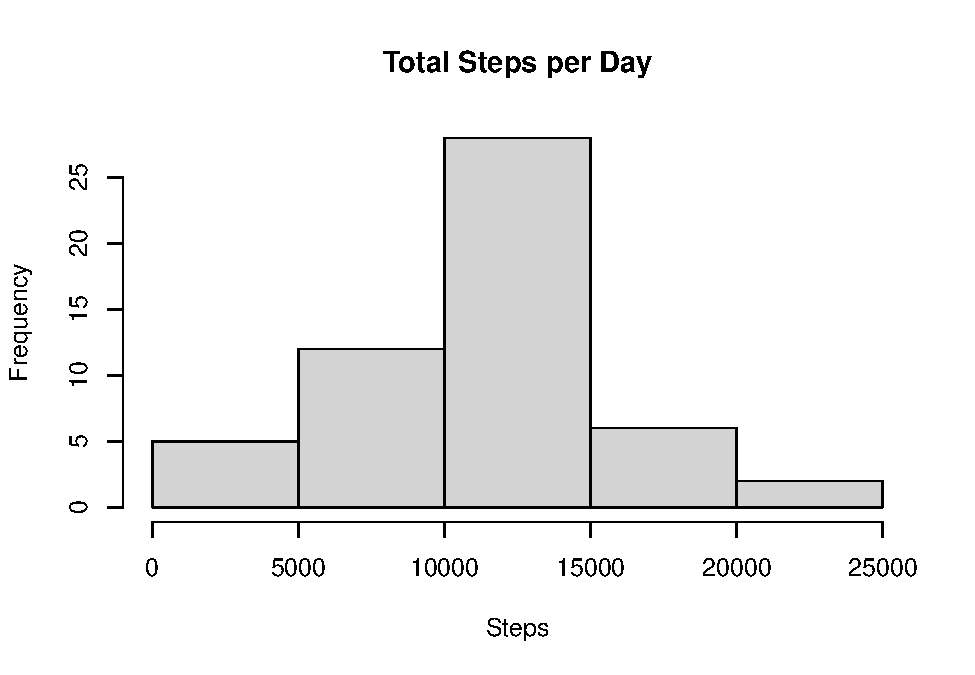
\includegraphics{project_1_files/figure-latex/daily_total-1.pdf}

Calculate and report the mean and median of the total number of steps
taken per day

\begin{Shaded}
\begin{Highlighting}[]
\FunctionTok{as.integer}\NormalTok{(}\FunctionTok{mean}\NormalTok{(sumTable}\SpecialCharTok{$}\NormalTok{Steps))}
\end{Highlighting}
\end{Shaded}

\begin{verbatim}
## [1] 10766
\end{verbatim}

\begin{Shaded}
\begin{Highlighting}[]
\FunctionTok{as.integer}\NormalTok{(}\FunctionTok{median}\NormalTok{(sumTable}\SpecialCharTok{$}\NormalTok{Steps))}
\end{Highlighting}
\end{Shaded}

\begin{verbatim}
## [1] 10765
\end{verbatim}

\hypertarget{what-is-the-average-daily-activity-pattern-1}{%
\subsection{What is the average daily activity
pattern?}\label{what-is-the-average-daily-activity-pattern-1}}

We need two: 1- Make a time series plot 2- Which 5-minute interval, on
average across all the days in the dataset, contains the maximum number
of steps?

\begin{Shaded}
\begin{Highlighting}[]
\CommentTok{\#import libraries}
\FunctionTok{library}\NormalTok{(plyr)}
\FunctionTok{library}\NormalTok{(ggplot2)}

\CommentTok{\#creating data}
\NormalTok{datos\_limpios }\OtherTok{\textless{}{-}}\NormalTok{ datos[}\SpecialCharTok{!}\FunctionTok{is.na}\NormalTok{(datos}\SpecialCharTok{$}\NormalTok{steps),]}

\CommentTok{\#creating average}
\NormalTok{Table\_inter }\OtherTok{\textless{}{-}} \FunctionTok{ddply}\NormalTok{(datos\_limpios, .(interval), summarize, }\AttributeTok{Avg=}\FunctionTok{mean}\NormalTok{(steps))}

\CommentTok{\#creating line plot}
\NormalTok{p }\OtherTok{\textless{}{-}} \FunctionTok{ggplot}\NormalTok{(Table\_inter, }\FunctionTok{aes}\NormalTok{(}\AttributeTok{x=}\NormalTok{interval, }\AttributeTok{y=}\NormalTok{Avg), }\AttributeTok{xlab=}\StringTok{"Interval"}\NormalTok{, }\AttributeTok{ylab =} \StringTok{"Average Numbwer of Steps"}\NormalTok{)}
\NormalTok{p }\SpecialCharTok{+} \FunctionTok{geom\_line}\NormalTok{() }\SpecialCharTok{+} \FunctionTok{xlab}\NormalTok{(}\StringTok{"Interval"}\NormalTok{) }\SpecialCharTok{+} \FunctionTok{ylab}\NormalTok{(}\StringTok{"Average Number of Steps"}\NormalTok{) }\SpecialCharTok{+} \FunctionTok{ggtitle}\NormalTok{(}\StringTok{"Average number of Steps per Interval"}\NormalTok{)}
\end{Highlighting}
\end{Shaded}

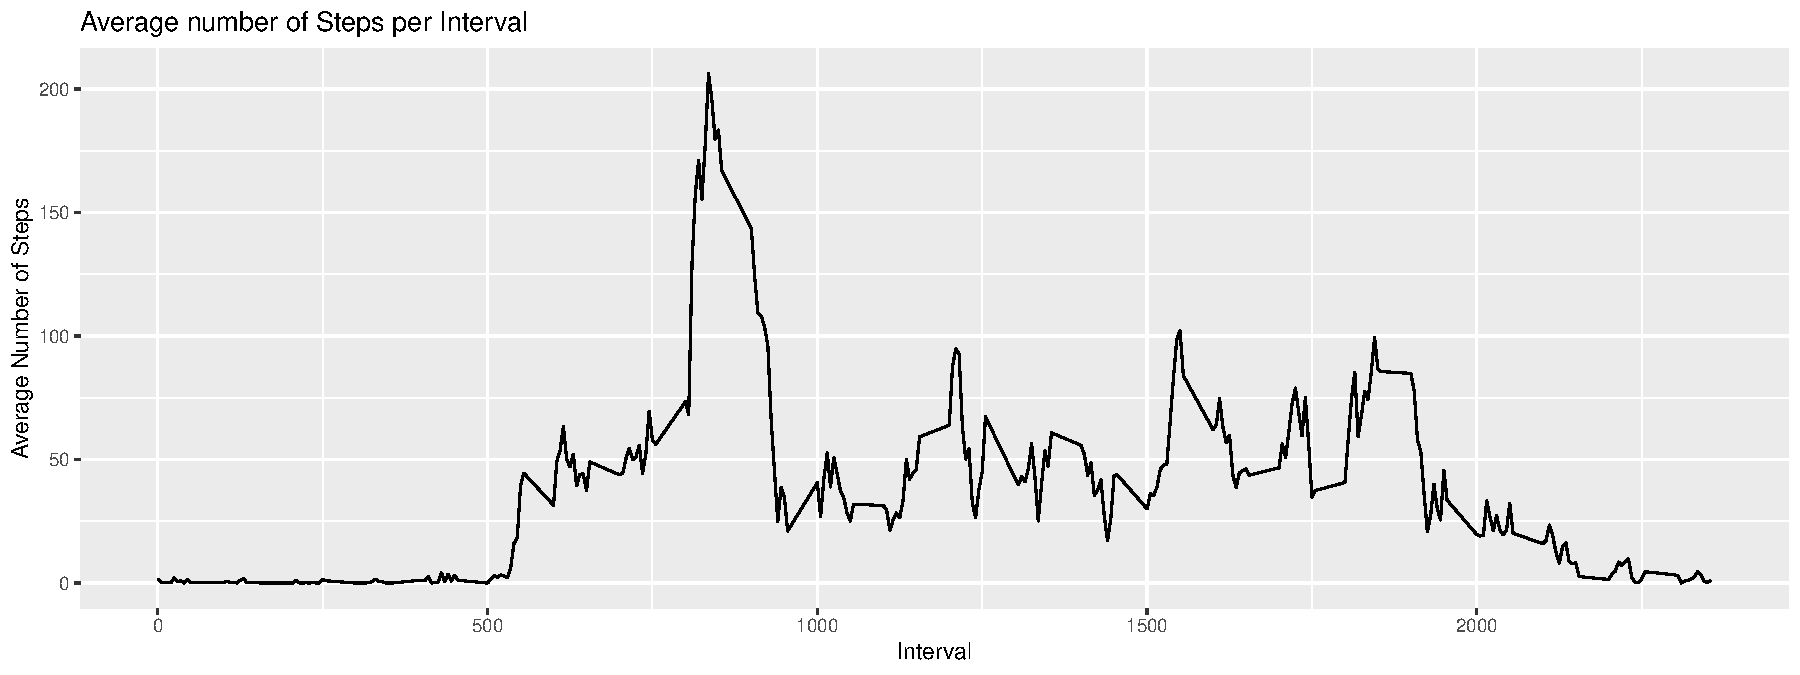
\includegraphics{project_1_files/figure-latex/daily-1.pdf}

\begin{Shaded}
\begin{Highlighting}[]
\DocumentationTok{\#\#Maximum steps by interval}
\NormalTok{maxSteps }\OtherTok{\textless{}{-}} \FunctionTok{max}\NormalTok{(Table\_inter}\SpecialCharTok{$}\NormalTok{Avg)}
\DocumentationTok{\#\#Which interval contains the maximum average number of steps}
\NormalTok{Table\_inter[Table\_inter}\SpecialCharTok{$}\NormalTok{Avg}\SpecialCharTok{==}\NormalTok{maxSteps,}\DecValTok{1}\NormalTok{]}
\end{Highlighting}
\end{Shaded}

\begin{verbatim}
## [1] 835
\end{verbatim}

\hypertarget{imputing-missing-values}{%
\subsection{Imputing missing values}\label{imputing-missing-values}}

Note that there are a number of days/intervals where there are missing
values (coded as \color{red}{\verb|NA|}NA). The presence of missing days
may introduce bias into some calculations or summaries of the data.

Calculate and report the total number of missing values in the dataset
(i.e.~the total number of rows with \color{red}{\verb|NA|}NAs)

Devise a strategy for filling in all of the missing values in the
dataset. The strategy does not need to be sophisticated. For example,
you could use the mean/median for that day, or the mean for that
5-minute interval, etc.

Create a new dataset that is equal to the original dataset but with the
missing data filled in.

Make a histogram of the total number of steps taken each day and
Calculate and report the mean and median total number of steps taken per
day. Do these values differ from the estimates from the first part of
the assignment? What is the impact of imputing missing data on the
estimates of the total daily number of steps?

\hypertarget{calculate-and-report-the-total-number-of-missing-values-in-the-dataset-i.e.-the-total-number-of-rows-with-nas}{%
\paragraph{1. Calculate and report the total number of missing values in
the dataset (i.e.~the total number of rows with
NAs)}\label{calculate-and-report-the-total-number-of-missing-values-in-the-dataset-i.e.-the-total-number-of-rows-with-nas}}

\begin{Shaded}
\begin{Highlighting}[]
\CommentTok{\#Number of NAs in original data set}
\FunctionTok{nrow}\NormalTok{(datos[}\FunctionTok{is.na}\NormalTok{(datos}\SpecialCharTok{$}\NormalTok{steps),])}
\end{Highlighting}
\end{Shaded}

\begin{verbatim}
## [1] 2304
\end{verbatim}

The total number of rows with steps = `NA' equal to 2304

\hypertarget{devise-a-strategy-for-filling-in-all-of-the-missing-values-in-the-dataset}{%
\paragraph{2. Devise a strategy for filling in all of the missing values
in the
dataset}\label{devise-a-strategy-for-filling-in-all-of-the-missing-values-in-the-dataset}}

\begin{Shaded}
\begin{Highlighting}[]
\CommentTok{\# First, creating average number}
\NormalTok{Table\_avg }\OtherTok{\textless{}{-}} \FunctionTok{ddply}\NormalTok{(datos\_limpios, .(interval, day), summarize, }\AttributeTok{Avg=}\FunctionTok{mean}\NormalTok{(steps))}

\CommentTok{\#Second, creating dataset with all NAs for substitution}
\NormalTok{nadatos }\OtherTok{\textless{}{-}}\NormalTok{ datos[}\FunctionTok{is.na}\NormalTok{(datos}\SpecialCharTok{$}\NormalTok{steps),]}

\CommentTok{\#merge datas}
\NormalTok{nuevos\_datos }\OtherTok{\textless{}{-}} \FunctionTok{merge}\NormalTok{(nadatos, Table\_avg, }\AttributeTok{by =}\FunctionTok{c}\NormalTok{(}\StringTok{"interval"}\NormalTok{, }\StringTok{"day"}\NormalTok{))}
\end{Highlighting}
\end{Shaded}

\hypertarget{create-a-new-dataset-that-is-equal-to-the-original-dataset-but-with-the-missing-data-filled-in.}{%
\paragraph{3. Create a new dataset that is equal to the original dataset
but with the missing data filled
in.}\label{create-a-new-dataset-that-is-equal-to-the-original-dataset-but-with-the-missing-data-filled-in.}}

Below code is just to verify if process of imputing missing values
correctly preserved original values (lines with no NAs)

\begin{Shaded}
\begin{Highlighting}[]
\CommentTok{\#creating datas}
\NormalTok{nuevos\_datos2 }\OtherTok{\textless{}{-}}\NormalTok{ nuevos\_datos[,}\FunctionTok{c}\NormalTok{(}\DecValTok{3}\NormalTok{,}\DecValTok{4}\NormalTok{,}\DecValTok{1}\NormalTok{,}\DecValTok{2}\NormalTok{)]}
\FunctionTok{colnames}\NormalTok{(nuevos\_datos2) }\OtherTok{\textless{}{-}} \FunctionTok{c}\NormalTok{(}\StringTok{"steps"}\NormalTok{, }\StringTok{"date"}\NormalTok{, }\StringTok{"interval"}\NormalTok{, }\StringTok{"day"}\NormalTok{)}

\CommentTok{\#mergin datas}
\NormalTok{mergeData }\OtherTok{\textless{}{-}} \FunctionTok{rbind}\NormalTok{(datos\_limpios, nuevos\_datos2)}
\end{Highlighting}
\end{Shaded}

Making histogram\ldots. hard work,, jeje

\begin{Shaded}
\begin{Highlighting}[]
\CommentTok{\#sum of steps}
\NormalTok{sumTable2 }\OtherTok{\textless{}{-}} \FunctionTok{aggregate}\NormalTok{(mergeData}\SpecialCharTok{$}\NormalTok{steps}\SpecialCharTok{\textasciitilde{}}\NormalTok{ mergeData}\SpecialCharTok{$}\NormalTok{date, }\AttributeTok{FUN =}\NormalTok{ sum,)}
\FunctionTok{colnames}\NormalTok{(sumTable2) }\OtherTok{\textless{}{-}} \FunctionTok{c}\NormalTok{(}\StringTok{"Date"}\NormalTok{, }\StringTok{"Steps"}\NormalTok{)}

\CommentTok{\#Mean}
\FunctionTok{as.integer}\NormalTok{(}\FunctionTok{mean}\NormalTok{(sumTable2}\SpecialCharTok{$}\NormalTok{Steps))}
\end{Highlighting}
\end{Shaded}

\begin{verbatim}
## [1] 10766
\end{verbatim}

\begin{Shaded}
\begin{Highlighting}[]
\CommentTok{\#median}
\FunctionTok{as.integer}\NormalTok{(}\FunctionTok{median}\NormalTok{(sumTable2}\SpecialCharTok{$}\NormalTok{Steps))}
\end{Highlighting}
\end{Shaded}

\begin{verbatim}
## [1] 10765
\end{verbatim}

\begin{Shaded}
\begin{Highlighting}[]
\CommentTok{\#histogram}
\FunctionTok{hist}\NormalTok{(sumTable2}\SpecialCharTok{$}\NormalTok{Steps, }\AttributeTok{breaks=}\DecValTok{5}\NormalTok{, }\AttributeTok{xlab=}\StringTok{"Steps"}\NormalTok{, }\AttributeTok{main =} \StringTok{"Total Steps per Day with NAs Fixed"}\NormalTok{, }\AttributeTok{col=}\StringTok{"Black"}\NormalTok{)}
\FunctionTok{hist}\NormalTok{(sumTable}\SpecialCharTok{$}\NormalTok{Steps, }\AttributeTok{breaks=}\DecValTok{5}\NormalTok{, }\AttributeTok{xlab=}\StringTok{"Steps"}\NormalTok{, }\AttributeTok{main =} \StringTok{"Total Steps per Day with NAs Fixed"}\NormalTok{, }\AttributeTok{col=}\StringTok{"Grey"}\NormalTok{, }\AttributeTok{add=}\NormalTok{T)}
\FunctionTok{legend}\NormalTok{(}\StringTok{"topright"}\NormalTok{, }\FunctionTok{c}\NormalTok{(}\StringTok{"Imputed Data"}\NormalTok{, }\StringTok{"Non{-}NA Data"}\NormalTok{), }\AttributeTok{fill=}\FunctionTok{c}\NormalTok{(}\StringTok{"black"}\NormalTok{, }\StringTok{"grey"}\NormalTok{) )}
\end{Highlighting}
\end{Shaded}

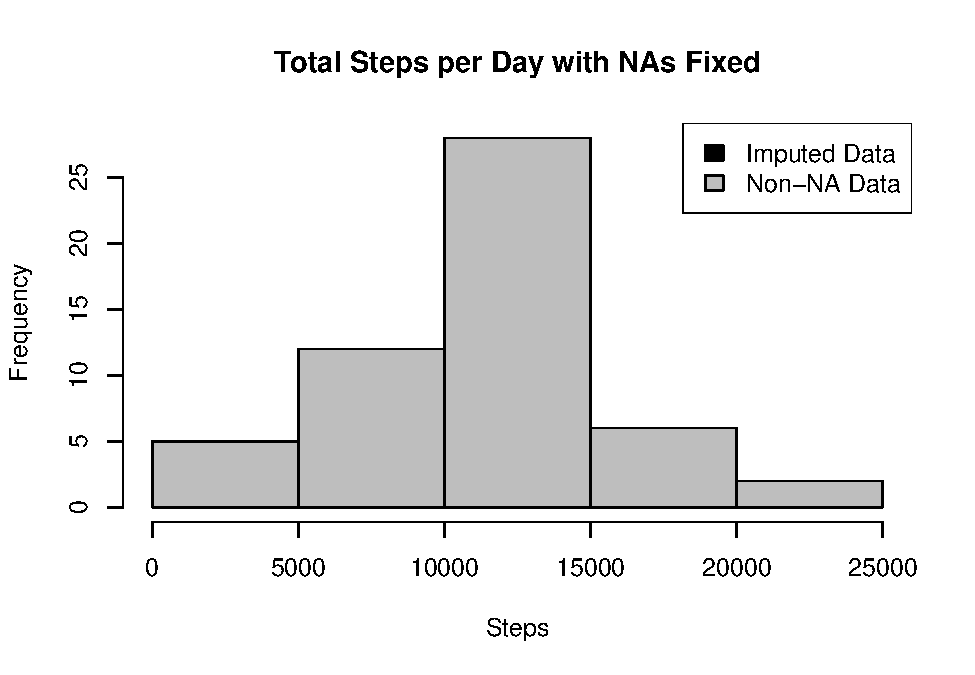
\includegraphics{project_1_files/figure-latex/unnamed-chunk-2-1.pdf}

\hypertarget{are-there-differences-in-activity-patterns-between-weekdays-and-weekends}{%
\subsection{Are there differences in activity patterns between weekdays
and
weekends?}\label{are-there-differences-in-activity-patterns-between-weekdays-and-weekends}}

\hypertarget{create-new-category-based-on-the-days-of-the-week}{%
\subsection{Create new category based on the days of the
week}\label{create-new-category-based-on-the-days-of-the-week}}

\begin{Shaded}
\begin{Highlighting}[]
\FunctionTok{library}\NormalTok{(lattice) }
\NormalTok{mergeData}\SpecialCharTok{$}\NormalTok{DayCategory }\OtherTok{\textless{}{-}} \FunctionTok{ifelse}\NormalTok{(mergeData}\SpecialCharTok{$}\NormalTok{day }\SpecialCharTok{\%in\%} \FunctionTok{c}\NormalTok{(}\StringTok{"Saturday"}\NormalTok{, }\StringTok{"Sunday"}\NormalTok{), }\StringTok{"Weekend"}\NormalTok{, }\StringTok{"Weekday"}\NormalTok{)}

\DocumentationTok{\#\# Summarize data by interval and type of day}
\NormalTok{intervalTable2 }\OtherTok{\textless{}{-}} \FunctionTok{ddply}\NormalTok{(mergeData, .(interval, DayCategory), summarize, }\AttributeTok{Avg =} \FunctionTok{mean}\NormalTok{(steps))}

\DocumentationTok{\#\#Plot data in a panel plot}
\FunctionTok{xyplot}\NormalTok{(Avg}\SpecialCharTok{\textasciitilde{}}\NormalTok{interval}\SpecialCharTok{|}\NormalTok{DayCategory, }\AttributeTok{data=}\NormalTok{intervalTable2, }\AttributeTok{type=}\StringTok{"l"}\NormalTok{,  }\AttributeTok{layout =} \FunctionTok{c}\NormalTok{(}\DecValTok{1}\NormalTok{,}\DecValTok{2}\NormalTok{),}
       \AttributeTok{main=}\StringTok{"Average Steps per Interval Based on Type of Day"}\NormalTok{, }
       \AttributeTok{ylab=}\StringTok{"Average Number of Steps"}\NormalTok{, }\AttributeTok{xlab=}\StringTok{"Interval"}\NormalTok{)}
\end{Highlighting}
\end{Shaded}

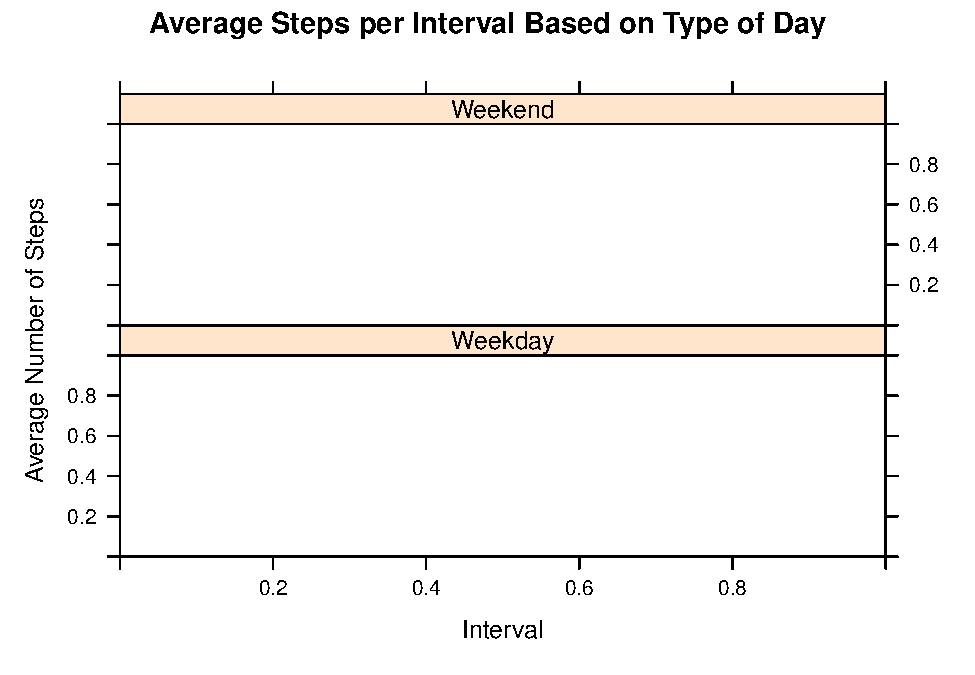
\includegraphics{project_1_files/figure-latex/unnamed-chunk-3-1.pdf}

\end{document}
